\section{Prise en main du LOGO}
%\subsection{Tutoriel vidéo}
\begin{UPSTIactivite}
    Cette activité permet la prise en main d'un automate LOGO. 

    Tout d'abord, visionner et suivre la \href{https://www.youtube.com/watch?v=ATcv0Dwm8ok}{vidéo} \url{https://www.youtube.com/watch?v=ATcv0Dwm8ok}.
    
    En utilisant des boutons poussoir au lieu des interrupteurs, réaliser le câblage proposé dans la vidéo et faire valider par l'enseignant. 
\end{UPSTIactivite}
\pagebreak

Le langage LADDER fut conçu dans les années 1970 pour faire passer les électrotechniciens de la saisie de schémas électriques de systèmes à relais  à la programmation.
Il est donc simple et proche de la description de schémas électriques.
On le réserve à la description de fonctions combinatoires ou à des calculs simples.

Une ligne d'un programme LADDER est appelée réseau.

Un réseau est composé de contacts, de bobine et/ou de blocs.

\subsection{Réseaux LADDER simples}

\subsubsection{Les contacts}

Les contacts représentent des entrées logiques (TOR).

\UPSTIaRetenir{Il existe deux types de contacts :
\begin{description}
  \item [$\begin{array}{l}\begin{tikzpicture}[circuit plc ladder,thick,x=\ladderskip,y=\ladderskip]
  \draw(0,0) to [contact NO={info={a}}] ++ (1,0);
\end{tikzpicture}
 \end{array}$] \textbf{Contact normalement ouvert} :
  actif lorsque la variable associée est à l'état 1.
  \begin{itemize}
    \item [$\Rightarrow$] Il représente donc la variable $a$
  \end{itemize}
  \item [$\begin{array}{l}\begin{tikzpicture}[circuit plc ladder,thick,x=\ladderskip,y=\ladderskip]
  \draw(0,0) to [contact NC={info={a}}] ++ (1,0);
\end{tikzpicture}
 \end{array}$]  \textbf{Contact normalement fermé } actif lorsque la variable associée est à l'état 0.
  \begin{itemize}
    \item [$\Rightarrow$] Il représente donc la variable $\overline{a}$
  \end{itemize}
\end{description}
}

\subsubsection{Les bobines}

Les bobines représentent les sorties logiques (TOR) de l'API.

\UPSTIaRetenir{Une sortie S de l'automate est active lorsque la bobine associée $\begin{array}{l}\begin{tikzpicture}[circuit plc ladder,thick,x=\ladderskip,y=\ladderskip]
  \draw(0,0) to [coil={info={S}}] ++ (1,0);
\end{tikzpicture}
\end{array}$ est active.}


\subsubsection{Réseaux de base}

La traduction en réseau LADDER de l'équation $S = a$ est donc représentée sur la figure \ref{fig:ladAtoS}. L'équation en réseau LADDER de l'équation $S = \overline{a}$ est représentée sur la figure~\ref{fig:ladABartoS}

\begin{figure}[ht]
  \begin{subfigure}[b]{.49\textwidth}
  \centering
    \begin{tikzpicture}[circuit plc ladder, thick, x=\ladderskip, y=\ladderskip]
  \draw(0,0) to [contact NO={info={a}}] ++ (1,0) -- ++(1,0)
    to [coil={info={Sortie}}] + (1,0) coordinate(laddertopright);
    \ladderrungend{1.2}
    \draw let \p1=(laddertopright) in
    (0,   \y1+0.7\ladderskip) -- (0,    \ladderskip)
    (\x1, \y1+0.7\ladderskip) -- (\x1,  \ladderskip);
\end{tikzpicture}

    \caption{$S = a$}
    \label{fig:ladAtoS}
  \end{subfigure}
  %
  \begin{subfigure}[b]{.49\textwidth}
  \centering
    \begin{tikzpicture}[circuit plc ladder, thick, x=\ladderskip, y=\ladderskip]
  \draw(0,0) to [contact NC={info={a}}] ++ (1,0) -- ++(1,0)
    to [coil={info={Sortie}}] + (1,0) coordinate(laddertopright);
    \ladderrungend{1.2}
    \draw let \p1=(laddertopright) in
    (0,   \y1+0.7\ladderskip) -- (0,    \ladderskip)
    (\x1, \y1+0.7\ladderskip) -- (\x1,  \ladderskip);
\end{tikzpicture}

    \caption{$S = \overline{a}$}
    \label{fig:ladABartoS}
  \end{subfigure}

  \caption{Réseaux LADDER de base}
\end{figure}

Comme dans un circuit électrique, il est possible de programmer des équation combinatoires en langage LADDER. Les fonctions \textbf{ET} et \textbf{OU} sont représentée sur la figure~\ref{fig:equaLogiques}

\begin{figure}[ht]
  \begin{subfigure}[b]{.49\textwidth}
    \centering
    \begin{tikzpicture}[circuit plc ladder, thick, x=\ladderskip, y=\ladderskip]
  \draw(0,0) to [contact NO={info={a}}] ++ (1,0)
    to [contact NO={info={b}}] ++ (1,0) -- ++(1,0)
    to [coil={info={Sortie}}] + (1,0) coordinate(laddertopright);
    \ladderrungend{1.2}
    \draw let \p1=(laddertopright) in
    (0,   \y1+0.7\ladderskip) -- (0,    \ladderskip)
    (\x1, \y1+0.7\ladderskip) -- (\x1,  \ladderskip);
\end{tikzpicture}

    \caption{$S = a \text{ ET } b$}
    \label{fig:aETb}
  \end{subfigure}
  %
  \begin{subfigure}[b]{.49\textwidth}
    \centering 
    \begin{tikzpicture}[circuit plc ladder,thick,x=\ladderskip,y=\ladderskip]
  \draw(0,0) to [contact NO={info={a}}] ++ (1,0) coordinate(laddercoil) -- ++(2,0) to [coil={info={Sortie}}] ++ (1,0) coordinate(laddertopright);
  \draw(0,-1) to [contact NO={info={b}}] ++ (1,0) -- (laddercoil);

  \ladderrungend{2}
  \draw let \p1=(laddertopright) in
  (0,   \y1+0.7\ladderskip) -- (0,    \ladderskip)
  (\x1, \y1+0.7\ladderskip) -- (\x1,  \ladderskip);
\end{tikzpicture}

    \caption{$S = a \text{ OU } b$}
    \label{fig:aOUb}
  \end{subfigure}
  \caption{Equations logiques simples}
  \label{fig:equaLogiques}
\end{figure}

\begin{UPSTIactivite}
    \UPSTIquestion{Dessinez le réseau LADDER de l'équation $S = a + \overline{b}$}

    \UPSTIlignesACompleter[2]{\begin{center}
      \input{ladder_diagrams/ladCircuitaOubBar.tikz}
    \end{center}}

    \UPSTIquestion{Dessinez le réseau LADDER de l'équation $S = \overline{a} \cdot \overline{b}$}

    \UPSTIlignesACompleter[2]{\begin{center}
      \begin{tikzpicture}[circuit plc ladder, thick, x=\ladderskip, y=\ladderskip]
  \draw(0,0) to [contact NC={info={a}}] ++ (1,0)
    to [contact NC={info={b}}] ++ (1,0) -- ++(1,0)
    to [coil={info={Sortie}}] + (1,0) coordinate(laddertopright);
    \ladderrungend{2}
    \draw let \p1=(laddertopright) in
    (0,   \y1+0.7\ladderskip) -- (0,    \ladderskip)
    (\x1, \y1+0.7\ladderskip) -- (\x1,  \ladderskip);
\end{tikzpicture}

    \end{center}}

    \UPSTIquestion{Dessinez le réseau LADDER de l'équation $S = (a + b) \cdot \overline{b} \cdot c $}

    \UPSTIlignesACompleter[2]{\begin{center}
      \begin{tikzpicture}[circuit plc ladder,thick,x=\ladderskip,y=\ladderskip]
  \draw(0,0) to [contact NO={info={a}}] ++ (1,0) coordinate(laddercoil)
  to [contact NC={info={b}}] ++ (1,0) 
  to [contact NO={info={c}}] ++ (1,0)
  -- ++(2,0) to [coil={info={Sortie}}] ++ (1,0) coordinate(laddertopright);
  \draw(0,-1) to [contact NO={info={b}}] ++ (1,0) -- (laddercoil);

  \ladderrungend{2}
  \draw let \p1=(laddertopright) in
  (0,   \y1+0.7\ladderskip) -- (0,    \ladderskip)
  (\x1, \y1+0.7\ladderskip) -- (\x1,  \ladderskip);
\end{tikzpicture}

    \end{center}}


\end{UPSTIactivite}


\pagebreak
\subsection{Application LADDER}
\begin{UPSTIactivite}[][LADDER]
    Soit le schéma suivant : 

    \begin{center}
        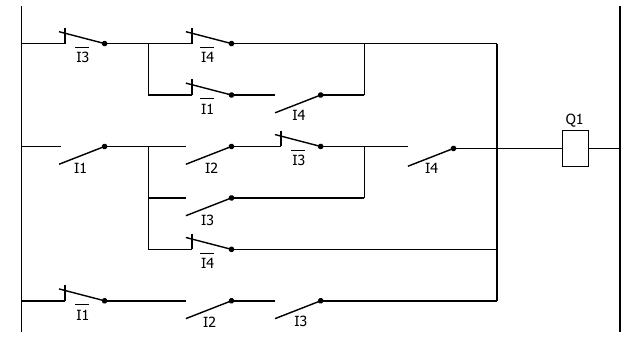
\includegraphics[width=.8\textwidth]{images/TP01_Ex01_cablage}
    \end{center}

    \begin{enumerate}
        \item Saisir ce schéma en LADDER dans LogoSoft
        \item A l'aide du simulateur, faire varier les entrées pour établir la table de vérité de la sortie Q1
        \item Transformer ce schéma en logigramme à l'aide de l'icone 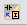
\includegraphics[height=\fontcharht\font`\B]{images/logoSoft_laderToSchema.png} et déterminer l'équation logique de la sortie Q1 
    \end{enumerate}
\end{UPSTIactivite}

\section{Exercice : Contrôle dimensionnel de pièces mécaniques}

\begin{figure}[ht]
    \centering
    \begin{subfigure}{0.49\textwidth}
        \centering
        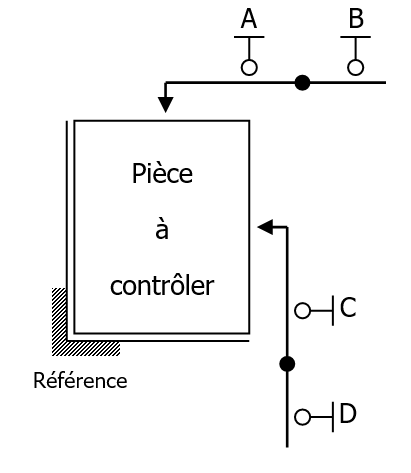
\includegraphics[width=\textwidth, height=.25\textheight, keepaspectratio]{images/TP01_Ex02_palpeur01}
        \caption{Pièce OK}
    \end{subfigure}
    \begin{subfigure}{0.49\textwidth}
        \centering
        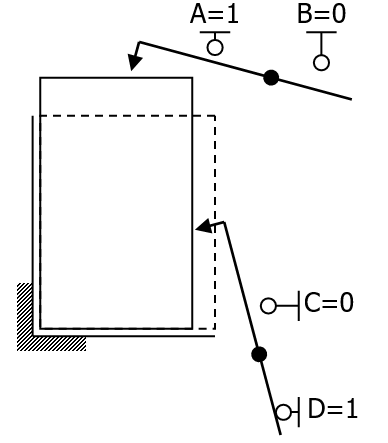
\includegraphics[width=\textwidth, height=.25\textheight, keepaspectratio]{images/TP01_Ex02_palpeur02}
        \caption{Pièce à rejeter}
    \end{subfigure}
    \caption{Palpeurs d'une pièce mécanique}
    \label{fig:palpeurs}
\end{figure}

Soit un système de contrôle dimensionnel de pièces mécaniques utilisant quatre capteurs A, B, C et D assoicés à deux palpeurs comme sur la Figure~\ref{fig:palpeurs}

Comme indiqué sur la Figure, les 4 capteurs sont inactifs pour une pièce de taille correcte. 

Le système de contrôle doit délivrer trois informations : 
\begin{description}
    \item[OK] lorsque la pièce est de taille correcte
    \item[Usinage] lorsque la pièce est trop grande sans qu'un côté soit trop petit
    \item[REJET] lorsque la pièce a au moins un côté trop petit  
\end{description}

\begin{table}[ht]
    \centering
    \begin{tabular}[]{c|c}
        Capteur & Entrée \\\hline
        A       &  I1\\
        B       &  I2\\
        C       &  I3\\
        D       &  I4\\
    \end{tabular}
    \caption{Correspondance Capteur - Entrée de l'automate}
\end{table}


\begin{UPSTIactivite}
    \UPSTIquestion{A l'aide de la Figure~\ref{fig:palpeurs}, donner les capteurs actifs lorsque la pièce est \begin{itemize}
        \item Trop haute
        \item Trop large
        \item Pas suffisamment hautre
        \item Pas suffisamment large
    \end{itemize}}

    %\UPSTIquestion{Etablir la table de vérité du système}
    \UPSTIquestion{Donner les équations de chaque sortie}
    \UPSTIquestion{Programmer le fonctionnement dans le langage de votre choix.}

    Les message seront affichés sur l'écran du LOGO : 
    \begin{itemize}
        \item OK sur fond BLANC
        \item USINAGE sur fond ORANGE
        \item REJET sur fond ROUGE 
    \end{itemize}
    \centering
    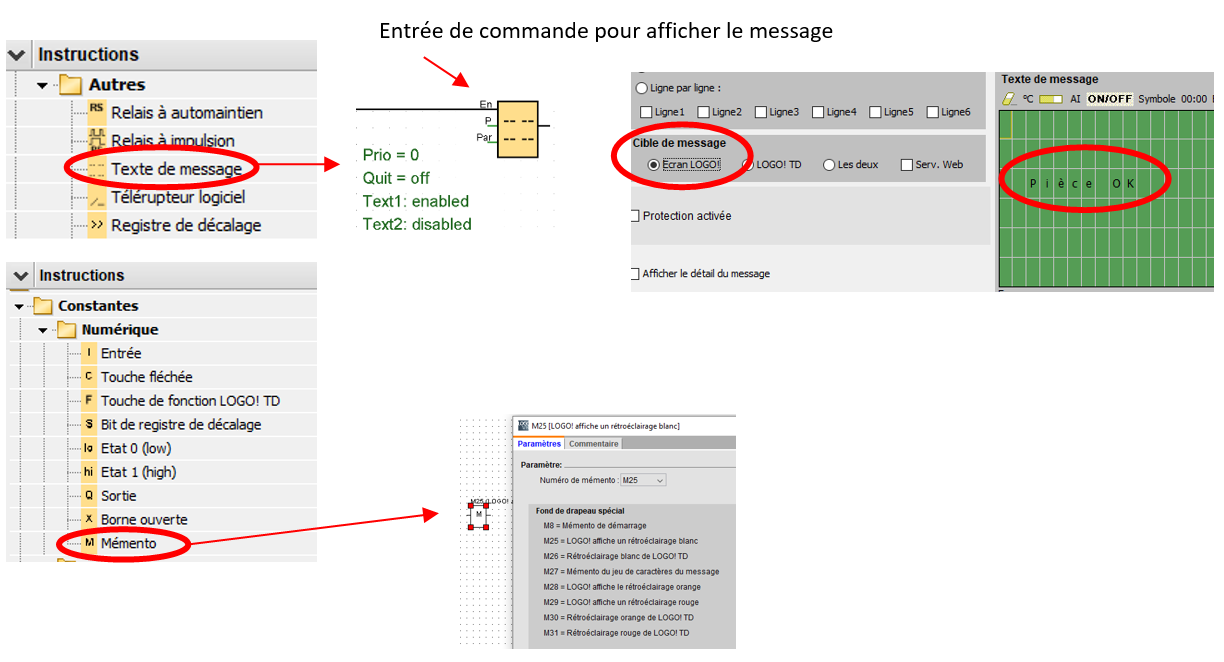
\includegraphics[width=.8\textwidth]{images/TP01_couleur_ecran.png}





\end{UPSTIactivite}